	Information theory provides one natural approach toward thinking about complex systems. It achieves this by mapping the physical concept of structure to the epistemic concept of predictability. A complex system has enough structure to be at least partially predictable, but enough disorder to make prediction challenging. In this paper, we apply information-theoretic tools to the measurement of \emph{spatial compositional complexity}, with a focus on the spatial variation of racial trends in American cities. 

	Information-theoretic concepts have already found application in urban planning problems related to zoning and predicting population distributions \cite{Royal2014,Batty1974,Batty1976,Battya}. Substantial recent work has addressed the measurement of difference and disparity in cities through an information-theoretic lens \cite{Theil1971,Bettencourt2015,Roberto2015a,Roberto2015}. Attractive features of information-theoretic measures for this purpose include their deep relationship to statistical inference \cite{Cover1991,Csiszzr2004}, their generalizability to multiple demographic phenomena, and the fact that Theil's (\cite{Theil1971}) original index satisfaction of many (though not all) of the invariance properties desirable for the measurement of segregation \cite{Reardon2002}. \nocite{Sampson2002,Dietz2002,Wong2004,Keeling1999,Anas1997,Ioannides2004a,Wong1999,Press2009a,Holloway2012,Lee2008,Louf2015}.

	While closely-related to segregation, the concept of complexity has received less attention among quantitative sociologists. This is natural, since complexity is both less operational than segregation and challenging to define. On the other hand, as we demonstrate below, a spatial information-theoretic measure can be defined which measures the granularity of neighborhood structure, distinguishing cities with large, monolithic tracts of constant racial composition from those with many adjacent, smaller, neighborhoods of varying racial profiles. In doing so, it therefore captures one natural aspect of complexity in spatial compositional phenomena, and may also be of interest as a segregation measure as well. 
	
\subsection{Information Theory and Spatial Structure}
	Two of the most fundamental objects of information theory are the entropy of a single random and the mutual information of two. Let $X$ be a spatial variable, such as a set of coordinates in space or a neighborhood name. Let $Y$ be a compositional variable that we aim to study, defined on an alphabet $\mathcal{Y}$. In the simple case in which $\mathcal{Y}  = \{\text{Black, White}\}$, Figure \ref{fig:toy} illustrates a range of possible joint distributions $p(X,Y)$. Comparing the completely undiverse city (a) and the spatially uniformly diverse (b) motivates the first fundamental information measure, the entropy:
	\begin{equation}
		H(Y) \triangleq \sum_{y \in \mathcal{Y}} p(y) \log p(y)\;.
	\end{equation}
	The entropy measures how evenly the global marginal distribution $p(Y)$ is distributed over the alphabet $\mathcal{Y}$. It thereby clearly distinguishes cities (a) and (b): since (a) is completely uniform, $H_a(Y) = 0$, while $H_b(Y) \neq 0$. On the other hand, the entropy $H$ is unable to distinguish between the spatial uniformity of (b) and the spatially variability of (c). To distinguish these two cities we may use the mutual information, which is defined in terms of the Kullback-Leibler divergence $D$:
	\begin{align}
		D[p(Z)\|q(Z)] &\triangleq \sum_z p(z) \log \frac{p(z)}{q(z)} \\
		I(X,Y) &\triangleq D[p(X,Y) \| p(X)p(Y)]
	\end{align}
	The divergence $D$ is (with some caveats) a measure of distance in the space of probability distributions, and so $I(X,Y)$ may be interpreted as the distance between the true joint distribution $p(X,Y)$ and the product of marginals $p(X)p(Y)$. Since the latter expresses statistical independence between $X$ and $Y$, $I(X,Y)$ measures the extent to which $X$ and $Y$ are dependent. In city (b), $X$ and $Y$ are independent: knowing $X$ (where an individual lives) conveys no information about that $Y$ (that individual's race).  In city (c), on the other hand $X$ and $Y$ are completely dependent: if you know where someone lives, you know their race with 100\% confidence. 

	City (d) shares with city (c) the fact that residence and race are maximally dependent. However, city (d) embodies the ``checkerboard problem'': measures that use only the joint distribution $p(X,Y)$ without additionally considering the spatial information contained within $X$ will evaluate city (d) to be the same as city (c), despite their considerably different patterns of racial separation and potentially very different implications for planning and policy. A recent working paper \cite{Roberto2015} provides one highly operational approach to this problem, using road network topology and a weighting function that decays with distance to define a localized measure based on the Kullback-Leibler divergence. Here we pursue an alternative strategy, showing that a localization of the mutual information both measures spatial variation in race and corresponds to the estimation of a fundamental statistical property of the distribution $p(X,Y)$. 


	\begin{figure}
		\centering
		  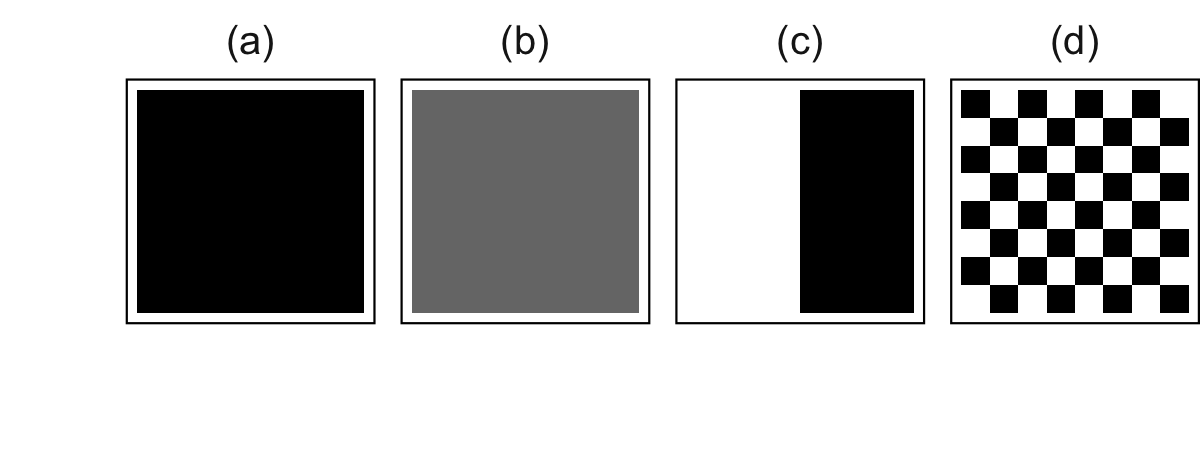
\includegraphics[width=.7\linewidth]{figs/checkerboard.png}
		  \begin{tabular}{c | c c c}
			  City & $H(Y)$ & $I(X,Y)$ & $J(X,Y)$ \\
			  \hline			
			  (a) & 0.0 & 0.0 & 0.0\\
			  (b) & 0.7 & 0.0 & 0.0\\
			  (c) & 0.7 & 0.7 & 0.6\\
			  (d) & 0.7 & 0.7 & 2.7\\
			  \hline  
			\end{tabular}
		\caption{Information theory and the checkboard problem: model cities with various kinds of spatial diversity can be distinguished through progressively more subtle spatial information measures.}
		\label{fig:toy}
		\end{figure}

